\section{Background}

\todo[inline]{Section introduction}

\subsection{Monitor Templates}
\noindent Monitor automata are utilized in my work to monitor the control flow of a given input source file and detect whether possible bug are present in this control flow. A monitor automaton will change state based on what is happening within the control flow of a program. When this monitor automaton reaches its final state, then a possible bug has been discovered. The effect analysis provided by EBA allows monitoring which effects program points have, and monitor automata can then monitor these effects in order to determine whether possible bugs are present. Effects within EBA happen on a region in the input program, and monitor automata must therefore monitor effects happening on a given region in order to determine whether effects happening on this region lead to possible bugs. It is, for example, common to have multiple locks on different regions within programs, but a lock on one region followed by a lock on a different region does not neccesarily mean that a bug is present. Regions, along with their effects, must therefore be monitored by these monitor automata. This can be expressed formally as follows. 

\newpar Given a region variable $\rho$, a monitor template is defined as the quintuple $X_\rho (\sum, S, s_0, \delta, F)$ where $\sum$ is the input alphabet, $S$ is a finite non-empty set of states happening on the region $\rho$, $s_0$ is an element of $S$ and initial state, $\delta$ is the state-transition function $\delta: S \times \sum \rightarrow S$ and $F$ is the possibly empty set of final states and a subset of $S$. An illustration of such a monitor automaton can be seen in Figure \ref{double-lock-automata-intro}.

\begin{figure}[H]
    \centering
    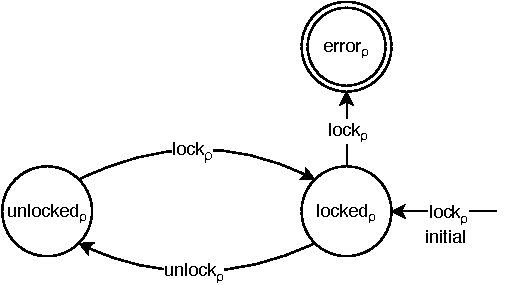
\includegraphics[width=0.5\textwidth]{background/figures/double-lock}
    \caption{An illustration of a monitor automaton.}
    \label{double-lock-automata-intro}
\end{figure}

\newpar Monitor automata operate on the set of possible effects of a statement in the Control-flow Graph, which are defined as $E = \{$\texttt{alloc}, \texttt{free}, \texttt{read}, \texttt{write}, \texttt{uninit}, \texttt{call}, \texttt{lock}, \texttt{unlock}$\}$ by Abal \cite{EffectiveBugFinding}, corresponding all possible variants of the $mem\_kind$ type defined previously. 

\newpar Monitor automata in this thesis all operate on a subset of $E$ and have a non-empty set of final states, $F$, indicating that a possible bug is discovered.  

\subsubsection{Double-unlock monitor automata}

\begin{figure}[H]
    \centering
    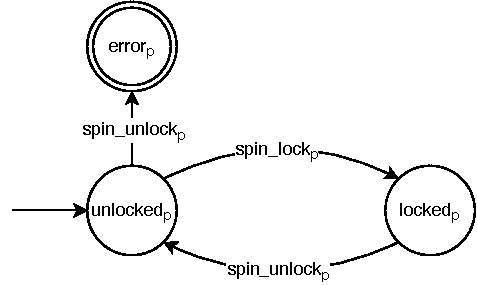
\includegraphics[width=0.5\textwidth]{background/figures/double-unlock}
    \caption{An illustration of a double-unlock monitor automata.}
    \label{double-unlock-automata}
\end{figure}

Given a region $\rho$, a double-unlock monitor automata is defined as the quintuple $(\sum, S, s_0, \delta, F)$ where: 

\begin{itemize}
    \item $\sum = \{\texttt{unlock}_\rho, \texttt{lock}_\rho\}$, a subset of $E$
    \item $S = \{ locked_\rho, unlocked_\rho, error_\rho \}$
    \item $s_0 = unlocked_\rho$ 
    \item $\delta =$ the relation $\{(locked_\rho, \texttt{unlock}_\rho, unlocked_\rho), (locked_\rho, \texttt{lock}_\rho, locked_\rho), \\
        (unlocked_\rho, \texttt{lock}_\rho, locked_\rho), (unlocked_\rho, \texttt{unlock}_\rho, error_\rho)\}$ 
    \item $F = error_\rho$  
\end{itemize}

An illustration of this monitor automata can be seen in Figure \ref{double-unlock-automata}. 

\newpar To show the detection of a possible double-unlock bug where a double-unlock monitor automaton has reached the final state, we find the product of the control flow example shown in Figure \ref{cfg_example-automaton} and the monitor generated from the template. 

\begin{itemize}
    \item{
        $
            \begin{aligned}[t] 
                \sum = & \{\mathit{Entry}, \mathit{Nil}, (alloc, \rho), (free, \rho), (read, \rho), \\ 
                & (write, \rho), (uninit, \rho), (call, \rho), (lock, \rho), (unlock, \rho)\}
            \end{aligned} 
        $
    }
    \item{
        $
            \begin{aligned}[t]
                S = & \{(allocated, \rho), (freed, \rho), (read, \rho), (written, \rho),\\ 
                & (uninitialized, \rho), (called, \rho), \\
                & ((locked, \rho), locked_\rho), ((unlocked, \rho), unlocked_\rho), \\
                & ((unlocked, \rho), error_\rho), \\
                & End\}
            \end{aligned}
        $
    }
    \item $s_0 = Entry$ 
    \item {
        $
            \begin{aligned}[t]
            \delta = \text{the relation} \; \{ \; & (Entry, (\texttt{alloc},\rho), (allocated, \rho)), \\ 
            & (allocated, (\texttt{alloc},\rho), (allocated, \rho)), \\ 
            & ((allocated, \rho), (\texttt{lock}, \rho), (locked, \rho)), \\
            & ((locked, \rho), (\texttt{unlock}, \rho), ((unlocked, \rho), unlocked_\rho), \\
            & (((unlocked, \rho), unlocked_\rho), \texttt{unlock}, ((unlocked, \rho), error_\rho)), \\ 
            & (((write, \rho), unlocked_\rho), \texttt{write}, ((written, \rho), unlocked_\rho)), \\ 
            & (((unlocked, \rho), error_\rho), \texttt{Nil}, (End, error_\rho)), \\ 
            & (((written, \rho), unlocked_\rho), \texttt{Nil}, (End, error_\rho)) \; \}
            \end{aligned}
        $ 
    }
    \item $F = (End, error_\rho)$  
\end{itemize}

\noindent This product can be illustrated as follows. 

\begin{figure}[H]
    \centering
    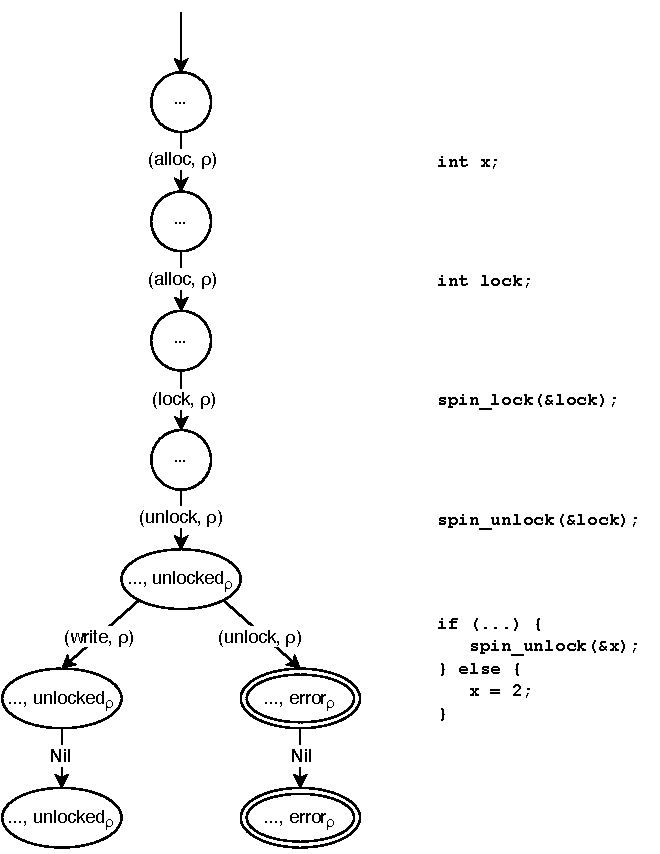
\includegraphics[width=0.5\textwidth]{background/figures/cfg_unlock-product}
    \caption{An illustration of the product construction of a double-unlock monitor automata and a control flow.}
    \label{cfg_unlock-product}
\end{figure}

\subsubsection{Double-lock monitor automata}

\begin{figure}[H]
    \centering
    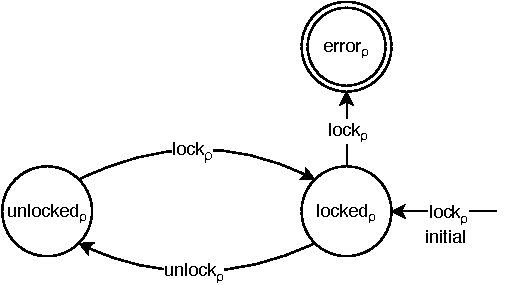
\includegraphics[width=0.5\textwidth]{background/figures/double-lock}
    \caption{An illustration of a double-lock monitor automata.}
    \label{double-lock-automata}
\end{figure}

Given a region $\rho$, a double-lock monitor automata is defined as the quintuple $(\sum, S, s_0, \delta, F)$ where: 

\begin{itemize}
    \item $\sum = \{\texttt{lock}_\rho, \texttt{unlock}_\rho\}$, a subset of $E$
    \item $S = \{ locked_\rho, unlocked_\rho, error_\rho \}$
    \item $s_0 = unlocked_\rho$ 
    \item $\delta =$ the relation $\{(unlocked_\rho, \texttt{lock}_\rho, locked_\rho), (locked_\rho, \texttt{unlock}_\rho, unlocked_\rho), \\
    (locked_\rho, \texttt{lock}_\rho, error_\rho), (unlocked_\rho, \texttt{unlock}_\rho, unlocked_\rho)\}$ 
    \item $F = error_\rho$  
\end{itemize}

An illustration of this monitor automata can be seen in Figure \ref{double-lock-automata}. 

\subsubsection{Double-free monitor automata}

\begin{figure}[H]
    \centering
    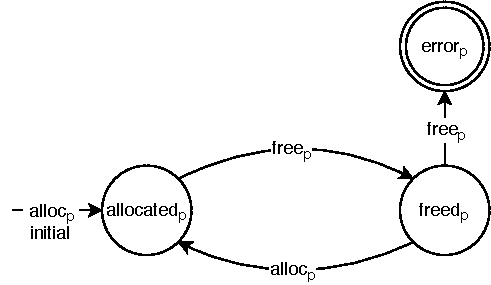
\includegraphics[width=0.5\textwidth]{background/figures/double-free}
    \caption{An illustration of a double-free monitor automata.}
    \label{double-free-automata}
\end{figure}

Given a region $\rho$, a double-free monitor automata is defined as the quintuple $(\sum, S, s_0, \delta, F)$ where: 

\begin{itemize}
    \item $\sum = \{\texttt{free}_\rho, \texttt{alloc}_\rho\}$, a subset of $E$
    \item $S = \{ allocated_\rho, freed_\rho, error_\rho \}$
    \item $s_0 = freed_\rho$ 
    \item $\delta =$ the relation $\{(freed_\rho, \texttt{alloc}_\rho, allocated_\rho), (allocated_\rho, \texttt{free}_\rho, freed_\rho), \\
    (freed_\rho, \texttt{free}_\rho, error_\rho), (allocated_\rho, \texttt{alloc}_\rho, allocated_\rho)\}$ 
    \item $F = error_\rho$  
\end{itemize}

An illustration of this monitor automata can be seen in Figure \ref{double-free-automata}. 

\subsubsection{Use-before-init monitor automata}

\begin{figure}[H]
    \centering
    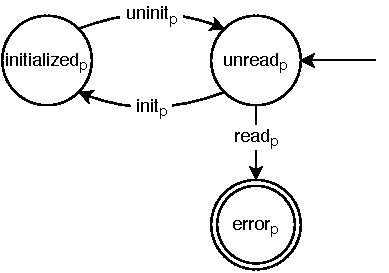
\includegraphics[width=0.5\textwidth]{background/figures/use-before}
    \caption{An illustration of a use-before-init monitor automata.}
    \label{use-before-automata}
\end{figure}

Given a region $\rho$, a use-before-init monitor automata is defined as the quintuple $(\sum, S, s_0, \delta, F)$ where: 

\begin{itemize}
    \item $\sum = \{\texttt{read}_\rho, \texttt{init}_\rho\}$, a subset of $E$
    \item $S = \{ unread_\rho, initialized_\rho, error_\rho \}$
    \item $s_0 = unused_\rho$ 
    \item $\delta =$ the relation $\{(unread_\rho, \texttt{init}_\rho, initialized_\rho), (initialized_\rho, \texttt{uninit}_\rho, unread_\rho), \\
    (unread_\rho, \texttt{read}_\rho, error_\rho), (initialized_\rho, \texttt{init}_\rho, initialized_\rho)\}$ 
    \item $F = error_\rho$  
\end{itemize}

An illustration of this monitor automata can be seen in Figure \ref{use-before-automata}. 

\subsection{Control Flow}

EBA provides a representation of the control flow of the input source files which is utilized in order to detect bugs. EBA generates a tree structure of the input, modeling statements as so-called \texttt{step}s. A path in this tree structure models a possible execution path, with each \texttt{step} in a path containing information about the modelled statements. A finite state machine is a quintuple $(\sum, S, s_0, \delta, F)$, where $\sum$ is an alphabet, $S$ is a finite non-empty set of states, $s_0$ is an element of $S$ and initial state, $\delta$ is the state-transition function $\delta: S \times \sum \rightarrow S$ and $F$ is the possibly empty set of final states and a subset of $S$. I will use such state machines to represent the code under analysis and the properties I wish to detect in input source files. 

The concrete tree structure modeling the resulting effects of statements can be formalized as the finite state machine $(\sum, S, s_0, \delta, F)$, where $\sum$ is the alphabet, $S$ is a finite non-empty set of states, $s_0$ is an element of $S$ and initial state, $\delta$ is the state-transition function $\delta: S \times \sum \rightarrow S$ and $F$ is the possibly empty set of final states and a subset of $S$. 

The control flow generated by EBA is acyclic, since EBA unrolls loops within a fixed depth and generates a path of this length accordingly. I keep the abstract formulation since, in principle, the monitor automata checkers will work with more general abstractions over programs.

The alphabet, $\sum$, of the of the control flow abstraction is the set of all effects EBA detects, annotated by the region variables being affected by a given effect. The states, $S$, are program points after the unrolling of loops. The definition of the control flow abstraction is shown in the following, with a concrete example of a control flow formulated using this abstraction in Figure \ref{cfg_example-automaton}. 

\begin{itemize}
    \item{
        $
            \begin{aligned}[t] 
                \sum = & \{\mathit{Entry}, \mathit{Nil}, (alloc, \rho), (free, \rho), (read, \rho), \\ & (write, \rho), (uninit, \rho), (call, \rho), (lock, \rho), (unlock, \rho)\}
            \end{aligned} 
        $
    }
    \item{
        $
            \begin{aligned}[t]
                S = & \{(allocated, \rho), (freed, \rho), (read, \rho), (written, \rho),\\ & (uninitialized, \rho), (called, \rho), (locked, \rho), (unlocked, \rho), End\}
            \end{aligned}
        $
    }
\end{itemize}

\noindent The remainder of the automaton definition is defined according to the control flow being modelled, where the initial state, $s_0$, is dependent on the control flow being modelled and therefore is an element of $\sum$. This also applies to the transition function $\delta$ and the set of final states $F$, which is also a subset of $\sum$. A concrete definition of an example control flow is shown below with an accompanying illustration of this in Figure \ref{cfg_example-automaton}.

\begin{figure}[H]
    \centering
    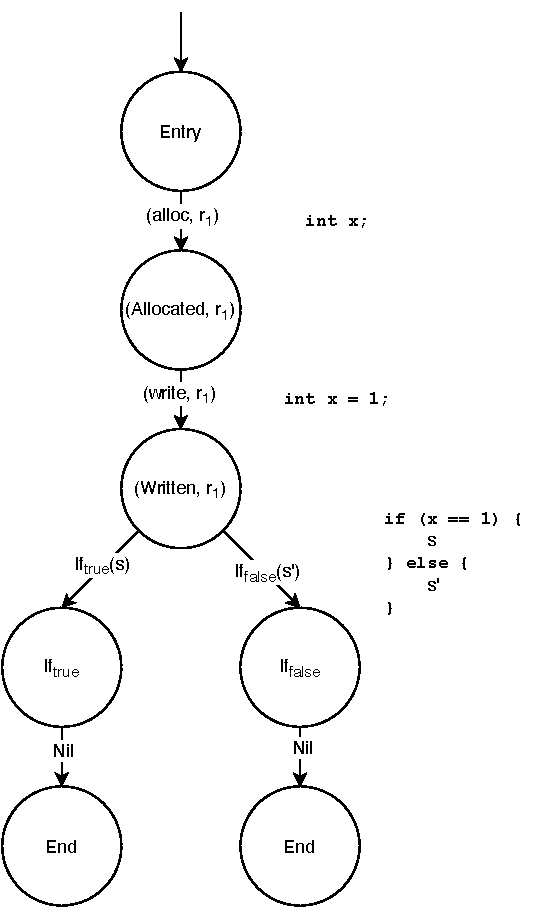
\includegraphics[width=0.5\textwidth]{background/figures/cfg_example}
    \caption{An illustration of a Control Flow automaton.}
    \label{cfg_example-automaton}
\end{figure}

\begin{itemize}
    \item $s_0 = Entry$ 
    \item {
        $
            \begin{aligned}[t]
            \delta = \text{the relation} \; \{ \; & (Entry, (\texttt{alloc},\rho), (allocated, \rho)), \\ 
            & (allocated, (\texttt{alloc},\rho), (allocated, \rho)), \\ 
            & ((allocated, \rho), (\texttt{lock}, \rho), (locked, \rho)), \\
            & ((locked, \rho), (\texttt{unlock}, \rho), (unlocked, \rho)), \\
            & ((unlocked, \rho), \texttt{unlock}, (unlocked, \rho), \\ 
            & ((write, \rho), \texttt{write}, (written, \rho)), \\ 
            & ((unlocked, \rho), \texttt{Nil}, End), \\ 
            & ((written, \rho), \texttt{Nil}, End) \; \}
            \end{aligned}
        $ 
    }
    \item $F = End$  
\end{itemize}

\noindent A few things are of note here; $Nil$ indicates the end of a path in the tree structure. Branches occur when an if-branch is encountered in the input source file and models the effects of the statements within if-statements.